\section{Portal by Example}
\label{sec:example}

In this section we illustrate the salient features of \ql, a
declarative query language for evolving graphs.  We will discuss how
\ql queries are evaluated in Section~\ref{sec:sys}.  We will use the
\tg \insql{T} of Figure~\ref{fig:tg}, with the structural schema
V(\underline{vid}:int, name:str, salary:int); E(\underline{vid1}:int,
\underline{vid2}:int, cnt:int), to develop our examples.

{\bf Temporal selection.}  Consider query $Q1$ below.  

\eat{
\begin{eqnarray*}
Q_1 & \insql{TSelect} & \insql{V ; E} \\
      & \insql{From} & \insql{T} \\
      & \insql{Start} & \insql{2010 End 2014}
\end{eqnarray*}
}

\begin{verbatim}
Q1: TSelect  V; E
    From     T
    Start    2010 End 2014
\end{verbatim}

$Q1$ performs temporal selection --- it's result is a \tg that
contains a consecutive subset of the snapshots of \insql{T}, namely,
$[2010, 2011)$ through $[2013, 2014)$, and has the same structural
    schema as \insql{T}.  The time period specified by the
    \insql{Start} \ldots \insql{End} clause is a closed-open period.
    Its time unit must match, or be coarser than, the time unit of
    \insql{T}. \reminder{What do we do if start or end falls within a
      snapshot, i.e., is not at the boundary?}

{\bf Specifying the structural schema of the result.  Analytics.}
Consider query $Q2$, which outputs a \tg with structural schema
V(\underline{vid}:int, bonus:float, pr:float) ;
E(\underline{vid1}:int, \underline{vid2}:int).

\begin{verbatim}
Q2: TSelect  V [vid, pagerank() as pr]; 
             E [vid1, vid2, cnt * 0.001 as score]
    From     T
\end{verbatim}

This query illustrates how the \insql{TSelect} clause can be used to
specify the structural schema of the result.  We may use this clause
to project out non-key columns of \insql{V} and \insql{E}, or to add
columns with computed values.  Data types of computed attributes
\insql{pr} and \insql{score} are determined by the return type of the
expression that computes them.  Note that key columns of \insql{V} and
\insql{E} must be present in the result.

The value of the attribute \insql{pr} in $Q2$ is computed using the
analytic function \insql{pagerank()}.  In addition to PageRank, \ql
supports a variety of analytic functions, including degree, shortest
path and connected component.  We provide an API that allows
developers to implement custom analytics that can either be computed
locally at a vertex, like degree, or that can be expressed in the
popular Pregel API. \reminder{Is what I'm saying true?  What other
  analytics do we support? How difficult is it to provide an API to
  support custom local / Pregel-style analytics?}

{\bf Temporal aggregation} is illustrated by query $Q3$, which, when
executed on \insql{T} from Figure~\ref{fig:tg}, computes the \tg in
Figure~\ref{fig:tg_any}.

\begin{verbatim}
Q3: TSelect   Any V ; Any E 
    From      T
    TGroup    by 2 years
\end{verbatim}


Temporal aggregation maps one or several consecutive snapshots from
the input to a single snapshot in the output.  How many input
snapshots are mapped to one snapshot in the output is specified in the
\insql{TGroup} clause.  Temporal aggregation in \ql is semantic, in
that we can aggregate an input \tg that has day as its unit into a \tg
with month as its time unit, by simply specifying \insql{TGroup by 1
  month}, and without having to worry about how many days there are in
a particular month.

Note the use of the modifier \insql{Any} in the \insql{TSelect} clause
of $Q3$.  This modifier specifies that the output contains a union of
the vertices (resp. edges) from the snapshots being aggregated.  In
our example, the snapshot $[2010, 2012)$ in the result s computed from
  snapshots $[2010, 2011)$ and $[2011, 2012)$ in the input and
      contains 5 vertices and 6 edges.

\begin{figure}
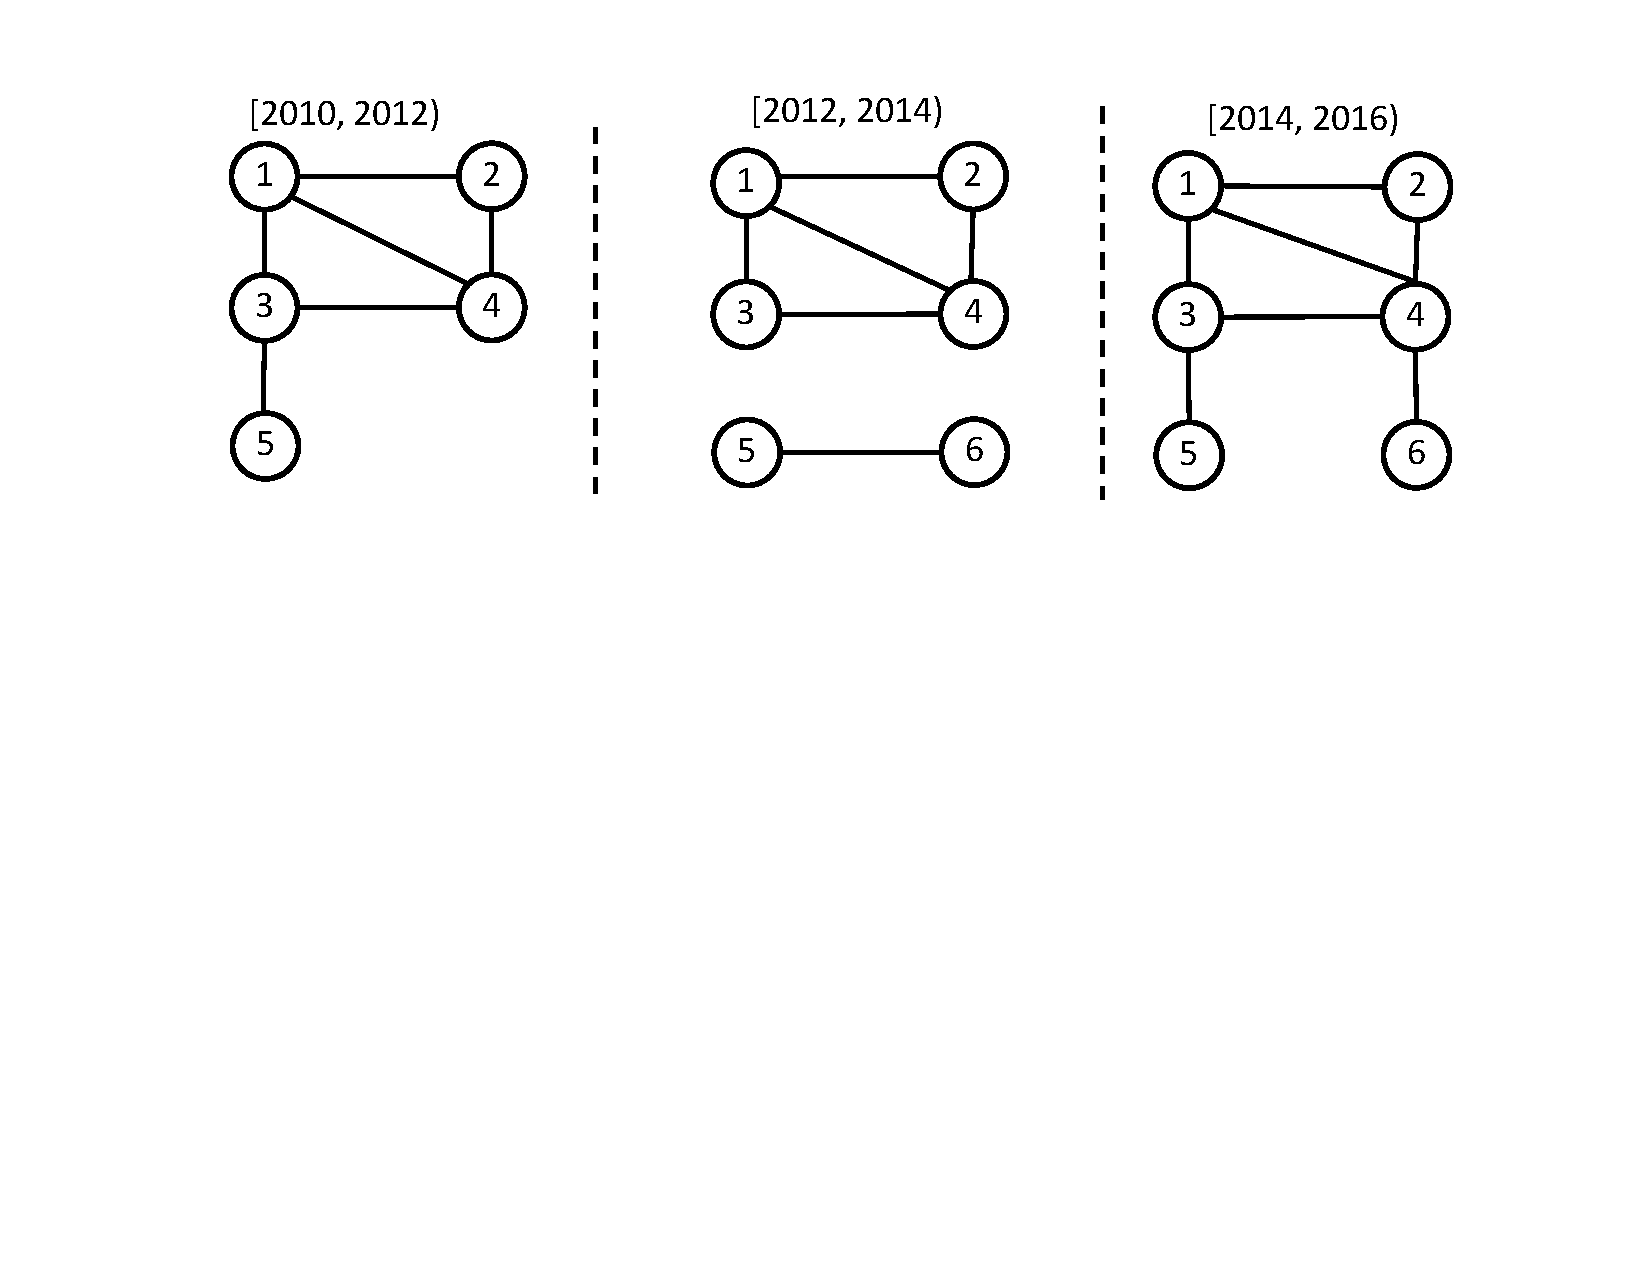
\includegraphics[width=3.2in]{figs/TGroupAny.pdf}
\caption{Result of query Q3.}
\label{fig:tg_any}
\end{figure}

Consider next query $Q4$, and its result in
Figure~\ref{fig:tg_all_any}.

\begin{verbatim}
Q4: TSelect All V [vid, any(name), max(salary)] ; 
            Any E [vid1, vid2, sum(cnt)] 
    From T 
    TGroup by 2 years
\end{verbatim}

The main difference between $Q4$ and $Q3$ is the \insql{All} modifier
associated with vertices in the \insql{TSelect} clause of $Q4$.
\insql{All V} states that the vertices in the result correspond to the
intersection of the vertices being aggregated.  \insql{Any E} states
that the edges in the result correspond to the union of the edges
connecting the vertices.  As our example illustrates, \insql{Any} and
\insql{All} modifiers are associated with vertices and edges and are
orthogonal, subject to the constraint that an edge can only be present
in a snapshot if both vertices it connects are present.

\begin{figure}
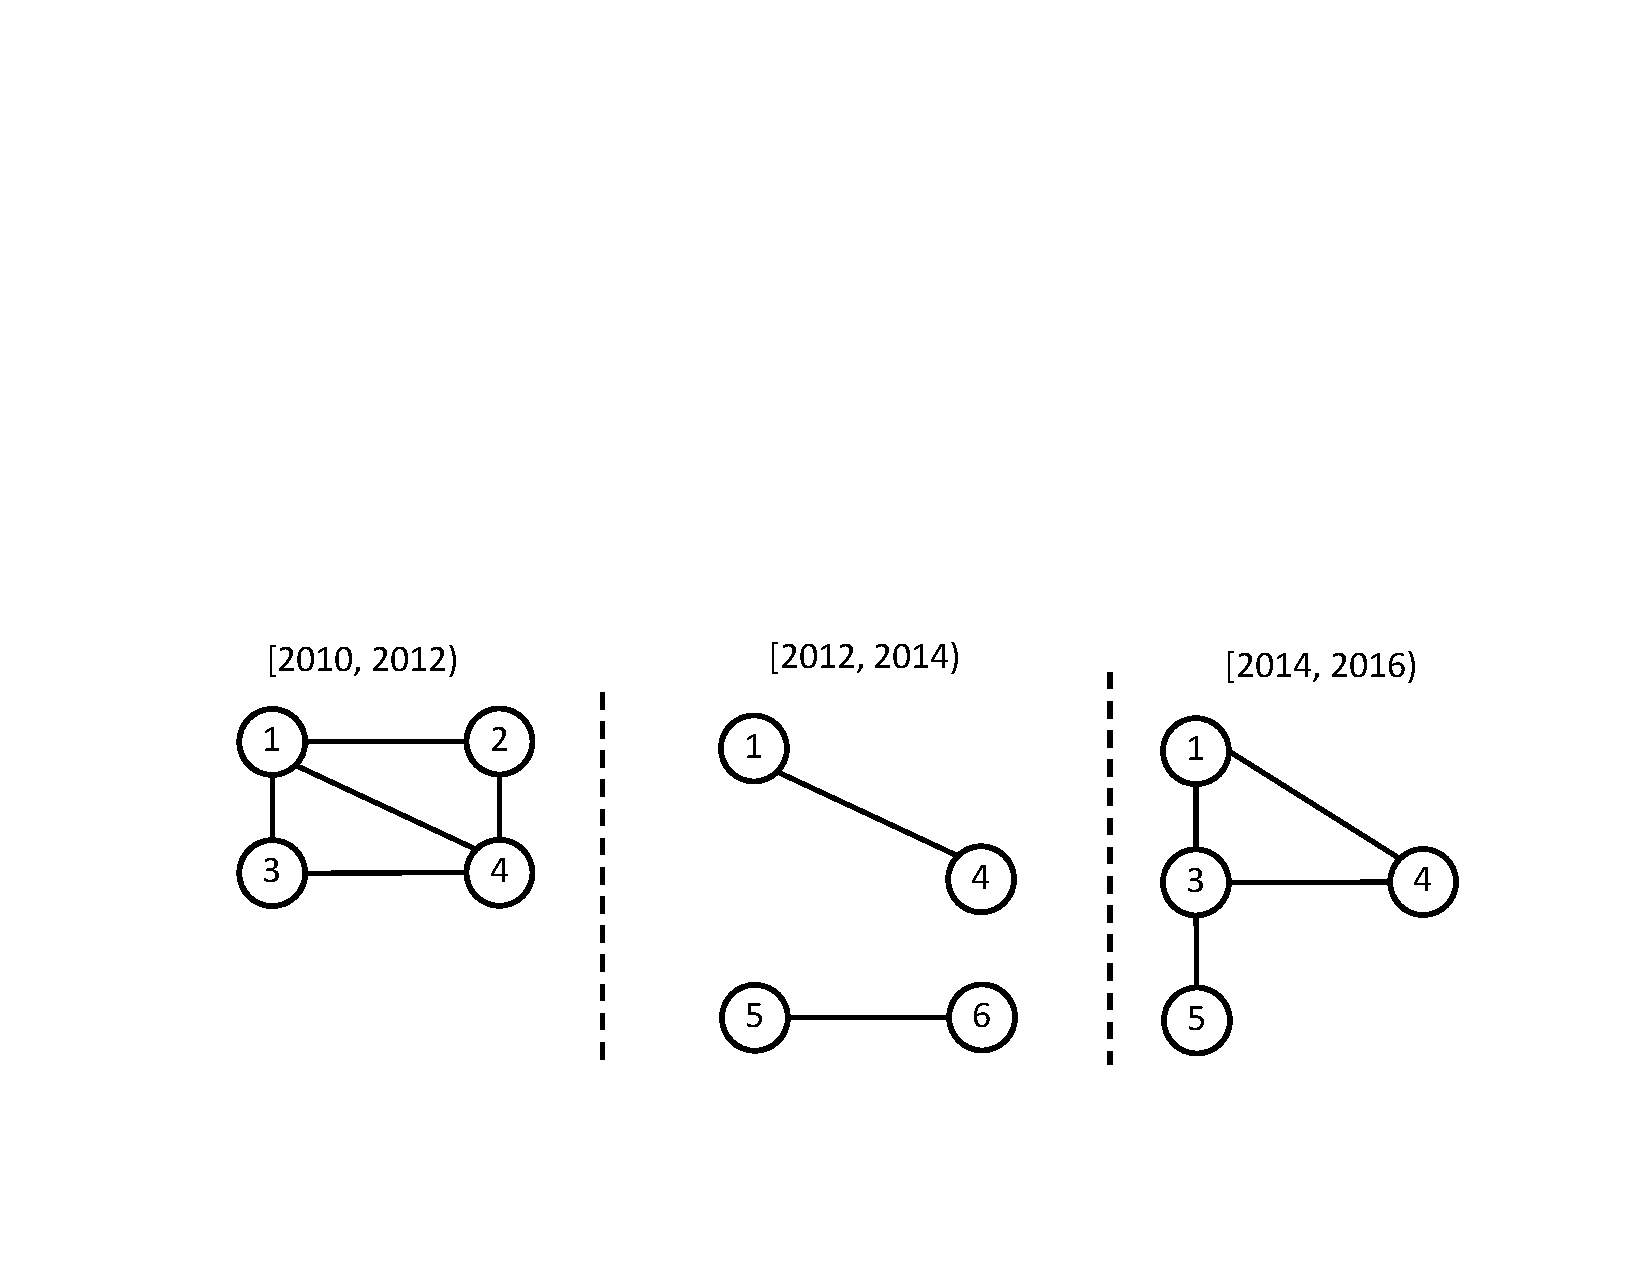
\includegraphics[width=3.2in]{figs/TGroupAllAny.pdf}
\caption{Result of query Q4.}
\label{fig:tg_all_any}
\end{figure}

$Q4$ illustrates another important feature of \ql, namely, aggregation
of values of non-key attributes of vertices and edges.  We make the
following aggregation operations available: \insql{any},
\insql{first}, \insql{last}, \insql{min}, \insql{max}, \insql{sum},
\insql{count}, and \insql{list}.

To illustrate, consider vertex and edge relations in
Figure~\ref{fig:2ve}, which correspond to the first two snapshots of
\insql{T}.  Vertex 1 is present in both $[2010, 2011)$ and $[2011,
    2012)$ in \insql{T}, and so is present in the snapshot $[2010,
      2012)$ of the result.  Vertex 1 has the same value for
      \insql{name} but different values for \insql{salary} in $[2010,
        2011)$ and $[2011, 2012)$.  Therefore, taking any value of
          \insql{name} and the maximum \insql{salary} may be
          appropriate.  Operations \insql{first} and \insql{last}
          return the value corresponding to the earliest
          (resp. latest) occurrence of the attribute, while
          \insql{list} returns a collection of all attribute values.

Returning to query $Q3$, when aggregation of attribute values is not
specified explicitly, \insql{any} is used as the default for non-key
attributes.  That is, the \insql{TSelect} clause of $Q3$ is short-hand
for \insql{TSelect Any V[vid, any(name), any(salary)] ;} 
\insql{Any E[vid1, vid2, any(cnt)]}.

In the current version of \ql, temporal aggregation always groups
\insql{V} and \insql{E} by their respective key attributes, and values
of all other attributes are aggregated with one of the provided
operators (\insql{any} being the default).  In the future we will
support grouping by non-key attributes, i.e., structural aggregation
of snapshots.  Further, we will define an API to allow developers to
specify custom aggregation operators.

{\bf Temporal intersection and union.} 

\begin{verbatim}
TSelect   Any V; Any E
From      T1 TOr T2
\end{verbatim}

\begin{verbatim}
  TSelect   Any V [id, any(name)]; Any E [id1, id2]
  From      T1 TAnd T2
  TGroup  by 2 years
\end{verbatim}

{\bf Combining operators.  Nested queries.}

\begin{verbatim}
  TSelect   Any V [id, any(name)]; Any E [id1, id2]
  From      (TSelect All V [id, any(name); 
                     All E [id1, id2, any(name)]
             From T1 TAnd T2
            )
  TGroup  by 2 years
\end{verbatim}

\begin{verbatim}
Q5  TSelect Any V [vid, any(name), max(salary)] ; 
            Any E [vid1, vid2, sum(cnt)]
    From      T
    TGroup    by 2 years
\end{verbatim}

\begin{verbatim}
  TSelect   Any V [id, any(name), max(salary), pagerank()];
            Any E   
  From      T
  Start     2000 End  2004
  TGroup    by 2 years
\end{verbatim}


\begin{verbatim}
  TSelect   All V[id, any(name), pagerank()]; 
            All E[id1, id2, sum(cnt)]
  From      T1 TAnd  
            (TSelect   Any V; Any E
             From      T1 TAnd T2)
  TGroup   by 2 years
\end{verbatim}

{\bf Loading data.  Inspecting results.}
